%!TEX root = ../dokumentation.tex

\chapter{Implementierung des Tools}

\section{Grundstruktur der Applikation}

Die Grundstruktur der Applikation basiert auf zwei im MATLAB App Designer erstellten Applikationen. Der Hauptapplikation, welche das Aufrufen einzelner Funktionalität ermöglicht, sowie den Graphen der erstellen Visualisierungen darstellt, und die Applikation zur Konfiguration der Samples, welche parallel zur Hauptapplikation als Pop-Up geöffnet werden kann, jedoch nicht ohne diese verwendbar ist. Als dritte Struktur wurde die sogenannte WithSamplesParser-Klasse erstellt, welche alle Funktionalitäten bezüglich der Messdatenverarbeitung und Darstellung enthält. Dazu gehören das Einlesend und Umstrukturieren der Messdaten auf ein passendes Format, sowie das Erstellen eines Graphen mit der passenden Konfiguration. Diese Funktionen werden dabei ebenfalls aus der Hauptapplikationen gestartet und benötigen diese deshalb auch als Grundlage.

\begin{figure}[!htbp]
	\centering
	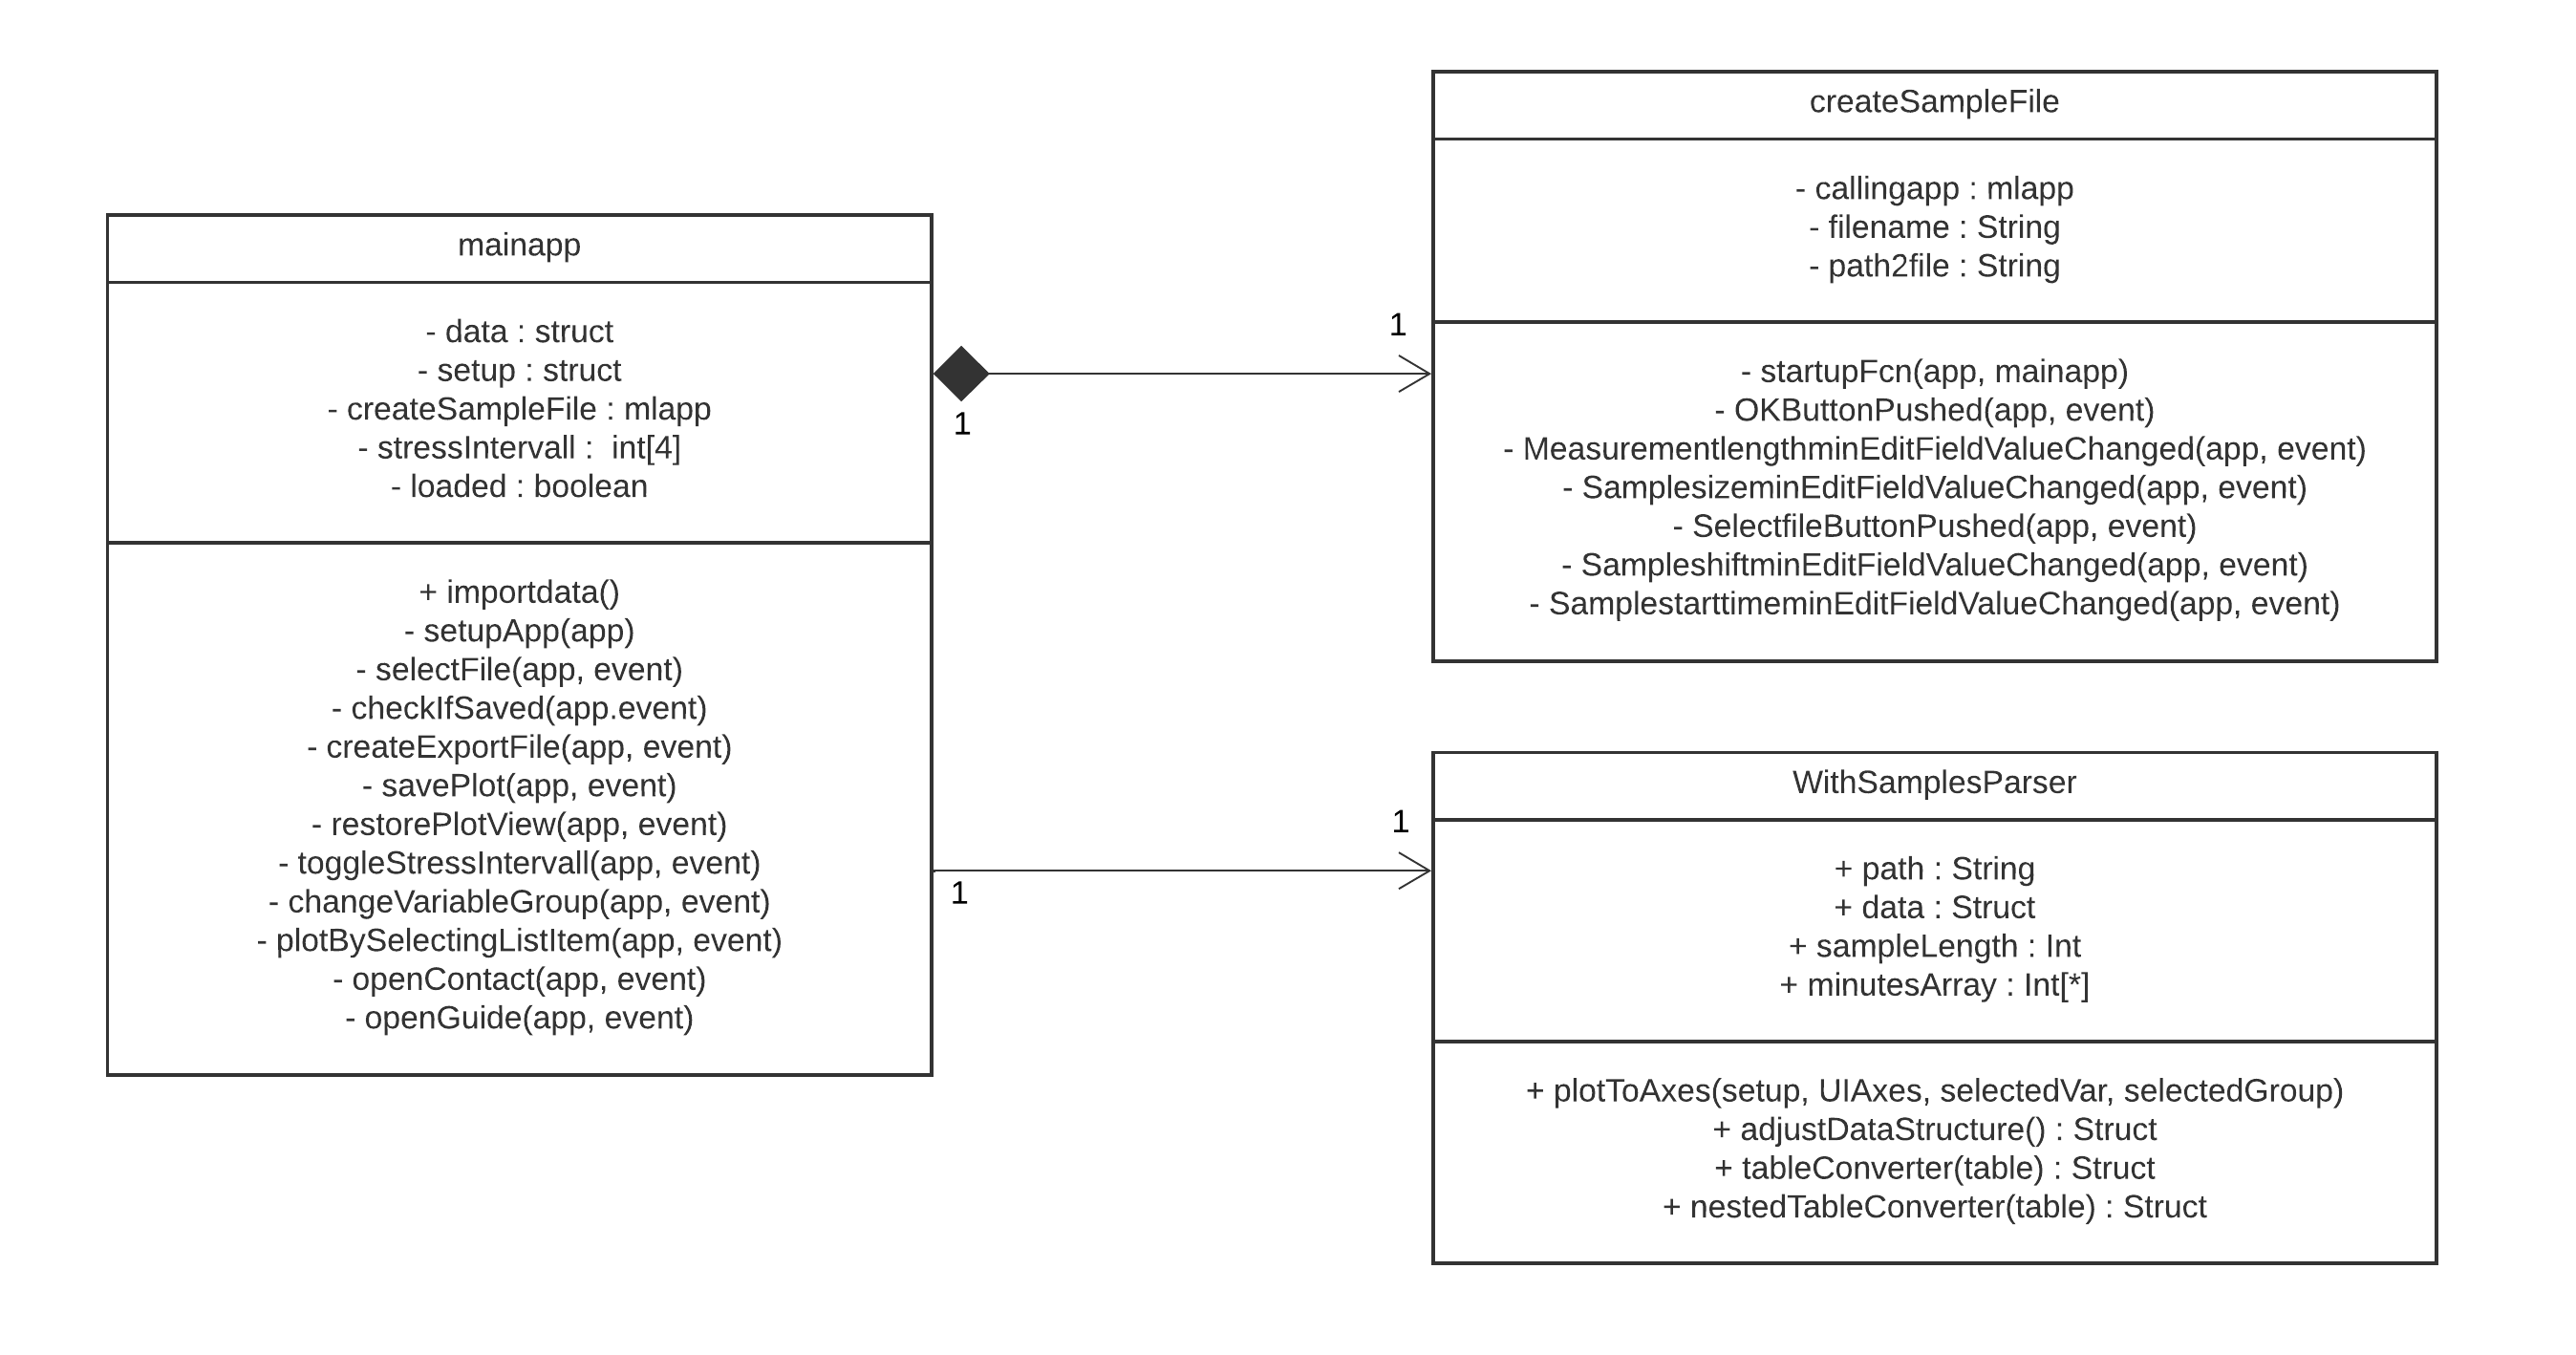
\includegraphics[width=1\linewidth]{klassendiagramm}
	\caption{Klassendiagramm der fertigen Applikation}
	\label{fig:klassendiagramm}
\end{figure}

\section{Erstellung der Samples}

% Tims Job

\section{Visualisierung der Daten}

Im folgenden Teil der Implementierung sollen die einzelnen Schritte und Funktionen dargestellt werden, welche zum schlussendlichen Visualisieren und Auswerten der Daten beitragen. Dazu gehören die Verarbeitung der Daten und die Datenstruktur im Backend der Applikation, sowie das Darstellen des Graphen mit Hilfe der Plot-Funktion und die dazugehörigen erweiternden Funktionen wie beispielsweise das Hervorheben des Belastungsintervalls.

\subsection{Datenstruktur und Datenverarbeitung}



% möglicherweise Datenstruktur als Baumdiagramm im Anhang anfügen

\subsection{Plot-Funktion}

\subsection{Zusätzliche Funktionen}